\documentclass[10pt]{beamer}

\usepackage{graphicx}

\usepackage[backend=biber]{biblatex}
\addbibresource{references.bib}

\title{Modelling Physical Phenomena, Planetary Motion and Conservation Laws}
\author{Gokulraj R - 2020102042 \\
Anjali Singh - 2020102004\\
Shruti Kolachana - 2020102053
}

\usetheme{Antibes}

\begin{document}

\maketitle

\begin{frame}
    \frametitle{Outline}
    \tableofcontents
\end{frame}

\section{Introduction}

\begin{frame}
    \frametitle{What is a Differential Equation?}
    \begin{itemize}
        \item A differential equation is an equation that related one or more unknown functions and their derivatives.
        \item In applications, the functions generally represent physical quantities, the derivatives represent their rate of changes, and the differential equation defines a relationship between the two.
        \item Two major division of differential equations: ODE and PDE.
    \end{itemize}
\end{frame}

\begin{frame}
    \frametitle{ODE and PDE}
    \begin{itemize}
        \item An ordinary differential equation (ODE) is an equation which has a dependent variable, which is an unknown function of an independent variable, its derivative, and some given functions of the independent variable.
        \item Examples for ODE: $y = x + \frac{dy}{dx}$, $(\frac{dy}{dx})^3 + \frac{d^2 x}{dy^2} - x \frac{dy}{dx} = y$, etc.
        \item A partial differential equation (PDE) is a differential equation that contains unknown multivariable functions and their partial derivatives.
        \item Examples for PDE: $\frac{\partial u}{\partial t} + t \frac{\partial u}{\partial x} = 0, \frac{\partial u}{\partial t} = 6u (\frac{\partial u}{\partial x})^2 - \frac{\partial ^3 u}{\partial x^3}$, etc.
    \end{itemize}

    \bigskip

    In this presentation, we only focus on modeling using ordinary differential equations.
\end{frame}

\begin{frame}
    \fontsize{9pt}{10pt}\selectfont
    \frametitle{Physical Quantities}
    \begin{itemize}
        \item Base or Fundamental Quantities:

            \quad \quad The quantities that are distinct in nature, which cannot be defined in terms of other quantities.

            \begin{enumerate}
                \item Length
                \item Time
                \item Mass
                \item Temperature
                \item Amount of substance
                \item Electric current
                \item Luminous Intensity
            \end{enumerate}

            \bigskip

        \item Other physical quantities can be defined using these base quantities (some function of base quantites).
        \item For instance, a derived physical quantity can be the rate of change of one quantity w.r.t another quantity (i.e., the derivative of one quanity w.r.t another), or the integral of one quantity w.r.t another quantity.
    \end{itemize}
\end{frame}

\section{Physical Phenomena}

\begin{frame}
    \frametitle{General Method to Model Physical Phenomena using Differential Equations}
    \begin{itemize}
        \item Assign variables to physical quantities.
        \item Some physical quantities will be functions (derivatives or integrals) of other physical quanitities related to the phenomena.
        \item Form equations using physical laws. These equations will be the differential equation model of the physical phenomena.
        \item The key to modeling is to choose the variables in such a way that the differential equations formed using the physical laws are simple to analyze.
        \item Now, the physical phenomena can be analyzed by analyzing the differential equations.
    \end{itemize}
\end{frame}

\begin{frame}
    \frametitle{In Kinematics}
    \begin{itemize}
        \item Displacement is usually denoted by the variable s.
        \item Velocity is the rate of change of displacement. i.e., $v = \frac{ds}{dt}$.
        \item Acceleration is the rate of change of velocity. i.e., $a = \frac{dv}{dt} = \frac{d^2s}{dt^2}$.
        \item Acceleration can also be written as $a = \frac{dv}{dt} = \frac{dv}{dt} \frac{ds}{ds} = v \frac{dv}{ds}$.
        \item These definitions are the most basic equations of kinematics. Every other relation is derived from them.
        \item Assuming $a$ is constant, solving the differential equations $a = \frac{dv}{dt}$, $v = \frac{ds}{dt}$ and $a = v \frac{dv}{ds}$, we get the equations of one dimensional motion with constant acceleration: $v = u + at$, $s = ut + \frac{1}{2}at^2$ and $v^2 - u^2 = 2as$, where $u$ denotes the initial velocity.
    \end{itemize}
\end{frame}

\begin{frame}
    \fontsize{9pt}{10pt}\selectfont
    \frametitle{Newtonian Mechanics}
    \begin{itemize}
        \item Momentum is defined as $p = mv$.
        \item Force is defined as the rate of change of momentum. i.e., $F = \frac{dp}{dt} = m \frac{dv}{dt}$ ($m$ is constant).
        \item Newton's Second Law: Net force acting on a body of mass $m$ is $F = m \frac{dv}{dt} = ma$.
        \item Work done is denoted by W and is defined as $W = Fs$. (more precisely, $dW = F ds$)
        \item NOTE: The quantities velocity, acceleration, momentum, force, etc are all vectors, althought here it is shown as a scalar (here, it is assumed for one dimensional physical systems). Work done is technically the dot product of $F$ and $s$.
        \item The work done on a body is stored as energy in it.
        \item Force can also be written as the anti-gradient of potential energy.
            $$
            F = - \frac{dU}{dx} \quad \textrm{(considering 1-D motion)}
            $$
    \end{itemize}
\end{frame}

\begin{frame}
    \frametitle{Example of a Mechanical System}
    Let us say a ball of mass $m$ is thrown vertically up in the air with an initial velocity of $u$ upward, where the viscous force coefficient is $b$ and the acceleration due to gravity is $g$ downward. Our goal is to find how the velocity and the position of the ball changes with time.
    \begin{itemize}
        \item Let the variable $x$ denote the position, $v$ denote the velocity and $a$ denote the acceleration of the ball at any instant $t$. Assume that the initial position of the ball as $x = 0$, and the positive axis directed upwards and the negative axis directed downwards.
        \item The force due to air friction (viscous force) at any instant is proportional to the magnitude of velocity ($bv$ in this case), directed opposite to the direction of the velocity.
        \item The other force acting on the ball is the gravitational force, which is $mg$ downward.
    \end{itemize}
\end{frame}

\begin{frame}
    \fontsize{9pt}{10pt}\selectfont
    \frametitle{Example of a Mechanical System (cont.)}
	\begin{columns}
		\column{0.3\textwidth}
        \begin{figure}
            \centering
            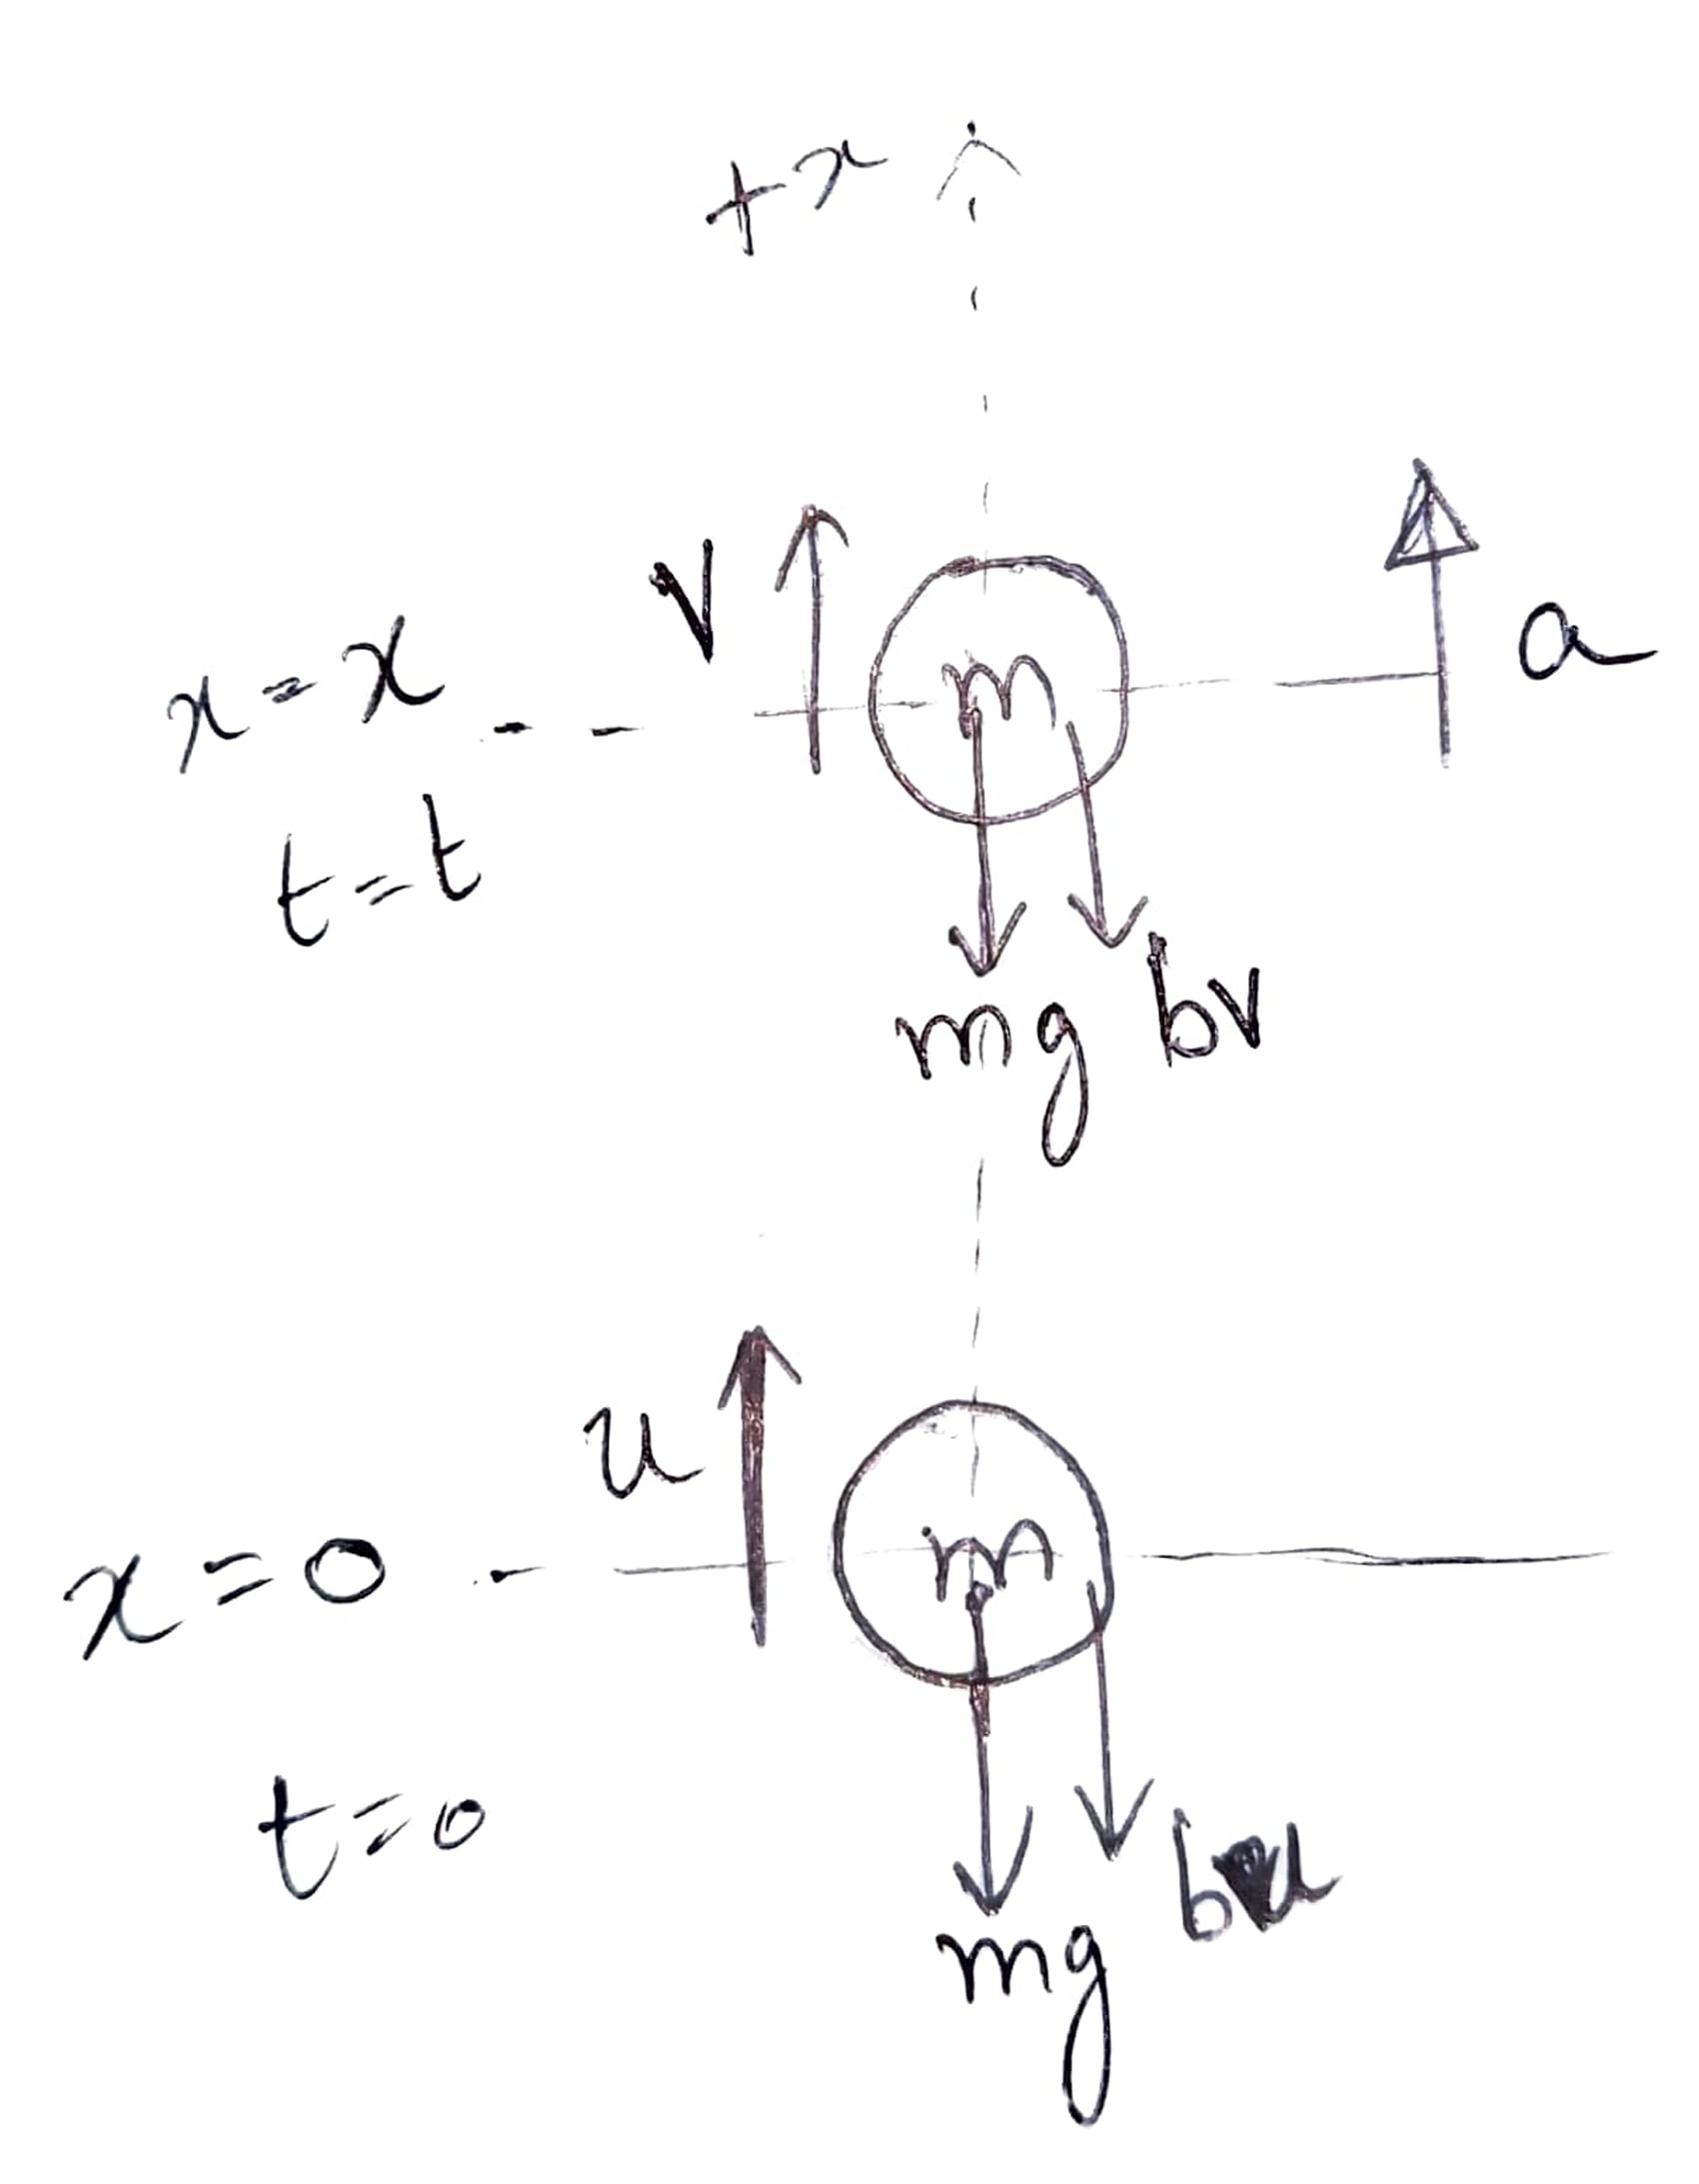
\includegraphics[height=0.6\textheight,width=\textwidth]{images/mechanics1.jpeg}
            \vfill
            \caption{Free-body diagram representing all the forces on the ball at any time $t$.}
            \label{fig:mechanics1}
        \end{figure}

		\column{0.7\textwidth}
        \begin{itemize}
            \item From Newton's second law, the net force on the ball at any instant must sum up to $ma$.
                $$
                -mg -bv = ma
                $$
                $$
                \implies-mg -bv = m \frac{dv}{dt}
                $$
            \item This is the differential equation that helps us find everything related to this system. Solving it by separating the variables and using the initial values, we get
                $$
                v = ue^{\frac{-bt}{m}} - \frac{mg}{b} (1 - e^{\frac{-bt}{m}})
                $$
            \item Once we have $v$ as a function of $t$, we can get $a$ and $x$ by differentiating and integrating $v$ w.r.t $t$ respectively.
        \end{itemize}

	\end{columns}
\end{frame}

\begin{frame}
    \frametitle{Electrostatics}
    \begin{itemize}
        \item Electric current ($i$) is defined as the rate of flow of charge ($q$). i.e., $i = \frac{dq}{dt}$.
        \item Defining electric charge in terms of the base quantity (electric current), $q = \int i dt$.
        \item Coulomb's Law: Force on an electric charge $q$ due to the charge $Q$ is given by $F = \frac{1}{4\pi\epsilon_0} \frac{Qq}{d^2}$, where $d$ is the distance between $Q$ and $q$.
        \item Electric field due to a point charge $Q$ at a point $d$ distance from it is defined as $E = \frac{1}{4\pi\epsilon_0} \frac{Q}{d^2}$.
        \item So, the electric force on a charge $q$ can also be written as $F = E q$, where $E$ is the electric field at that point due to all the other charges.
    \end{itemize}
\end{frame}

\begin{frame}
    \frametitle{Electrostatics}
    \begin{itemize}
        \item Electric potential due to a point charge $Q$ at a point $d$ distance from it is the work done in bringing an unit positive charge from infinity to the point at a distance $d$.

        \begin{center}
            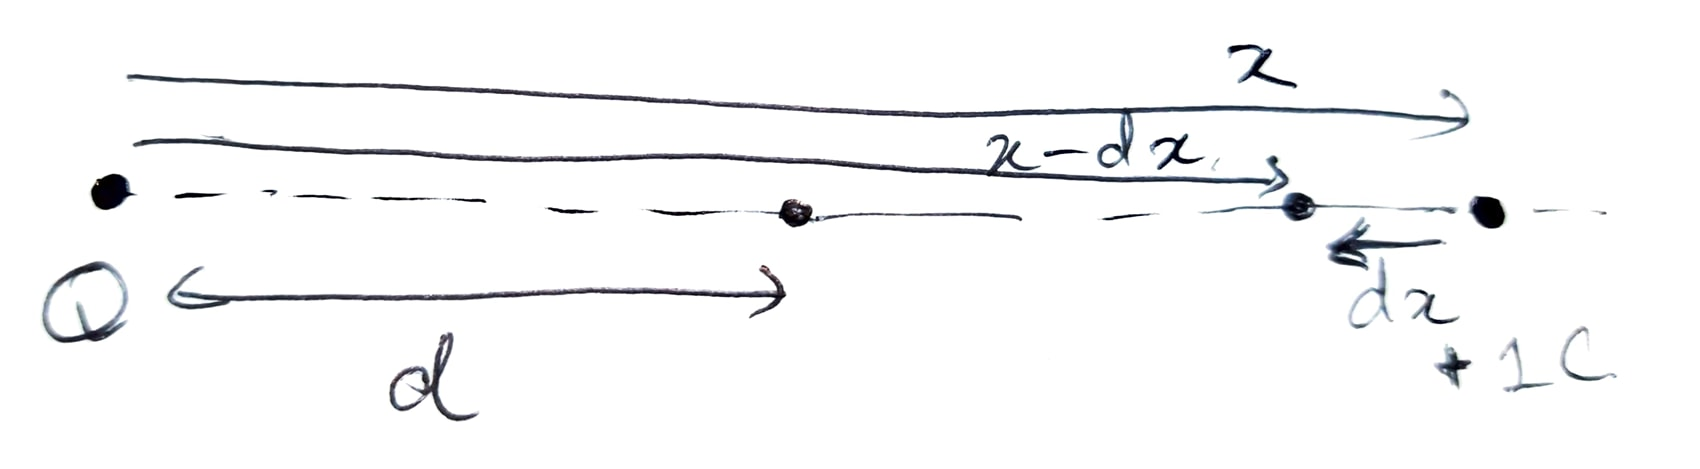
\includegraphics[height=0.2\textheight,width=0.5\textwidth]{images/electrostats_potential.jpeg}
        \end{center}
        \item Let $dW$ be the work done by the external force in moving the charge $+1C$ from $x$ to $x+dx$.
            $$
            dW = -F dx \implies dW = \frac{-1}{4\pi\epsilon_0} \frac{Q}{x^2} dx
            $$
        \item Integrating this from $x = \infty$ to $x = d$, we get the total work done, which is the required electric potential ($V$).
            $$
            V = \frac{1}{4\pi\epsilon_0} \frac{Q}{d^2}
            $$
    \end{itemize}
\end{frame}

\begin{frame}
    \frametitle{Modelling example in Electrostatics}
    Consider a line of charge of infinite length, with charge density $\lambda$ coulombs per unit length. Our goal is to find the magnitude of electric field due to the line of charge at a point $L$ distance from it.
    \begin{center}
        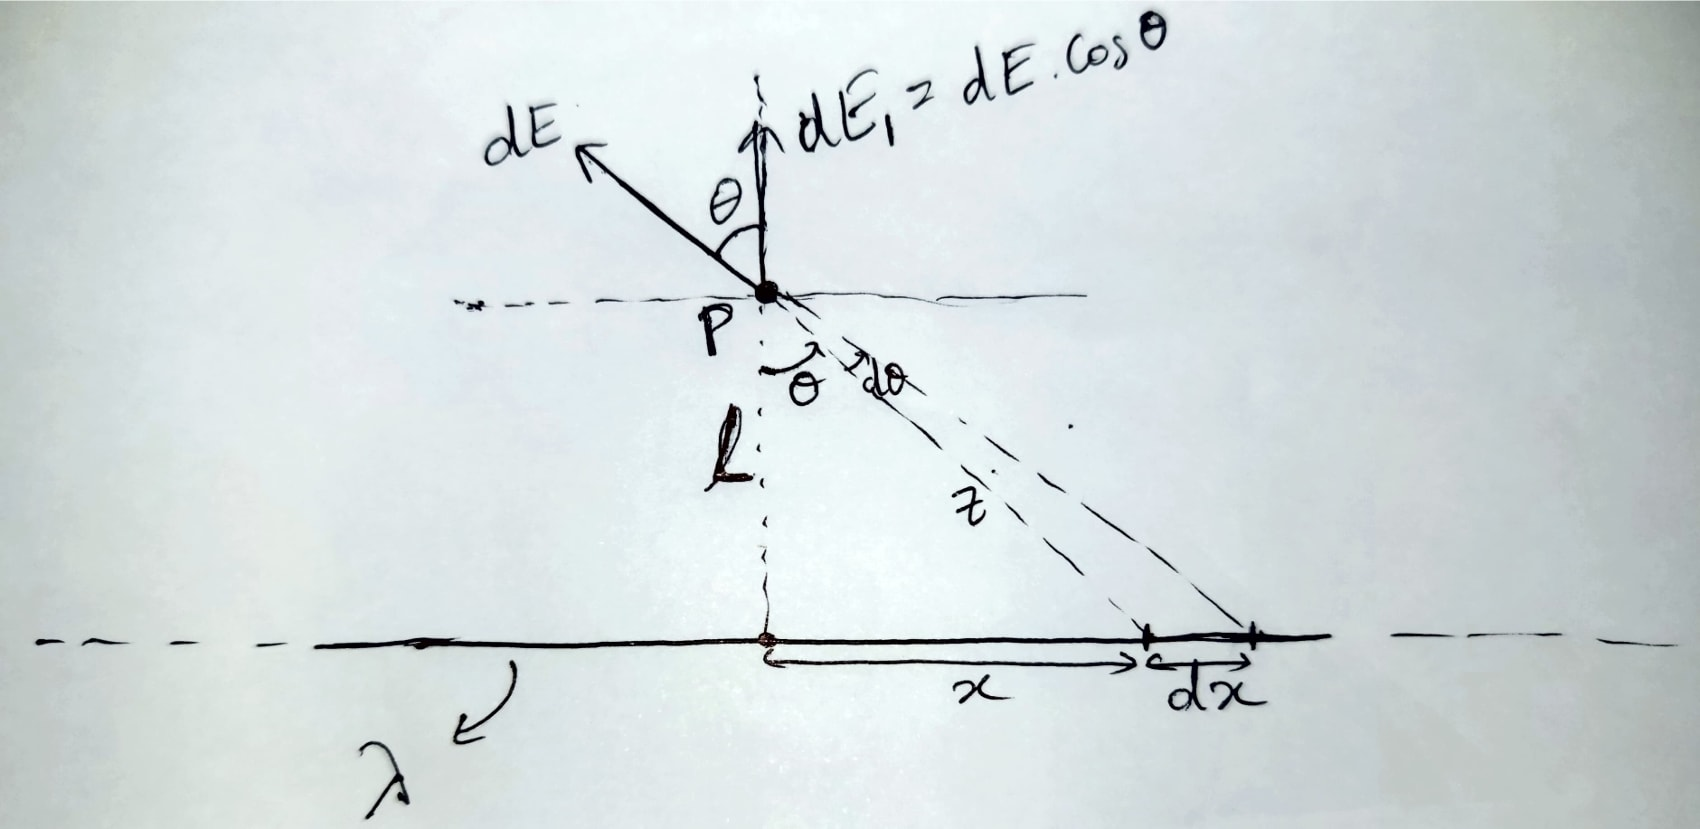
\includegraphics[height=0.2\textheight,width=0.4\textwidth]{images/electrostats_field_calc.jpeg}
    \end{center}
    \begin{itemize}
        \item Take a infinitesimal length $dx$ of the infinite line charge at a distance (or at an angle $\theta$ w.r.t the perpendicular about the point $P$).
        \item Let the electric field due to this small length be $dE$ (shown in the figure). The total electric field at P is the summation of the vertical components ($dE cos\theta$) of all such $dE$.
        \item The infinitesimal charge present in the length $dx$ is $\lambda dx$. The electric field due to this charge is $dE = \frac{1}{4\pi\epsilon_0} \frac{\lambda dx}{z^2}$.
    \end{itemize}
\end{frame}

\begin{frame}
    \frametitle{Modelling example in Electrostatics(cont.)}
    \begin{itemize}
        \item From the figure $z = \frac{L}{cos\theta}$ and $x = L (tan\theta) \implies dx = L (sec^2\theta) d\theta$.
            $$
            \implies dE = \frac{1}{4\pi\epsilon_0} \frac{\lambda L (sec^2\theta) d\theta}{\frac{L^2}{cos^2\theta}}
            $$
            $$
            \implies dE = \frac{1}{4\pi\epsilon_0} \frac{\lambda}{L} d\theta
            $$
        \item The total electric field at P is $\int dE_1 = \int dE (cos\theta)$.
            $$
            E_1 = \int_{\frac{-\pi}{2}}^{\frac{\pi}{2}} \frac{1}{4\pi\epsilon_0} \frac{\lambda}{L} cos\theta d\theta
            $$
            $$
            \boxed{E_1 = \frac{1}{2\pi\epsilon_0} \frac{\lambda}{L}}
            $$
    \end{itemize}
\end{frame}

\begin{frame}
    \fontsize{9pt}{10pt}\selectfont
    \frametitle{Electricity}
    \begin{itemize}
        \item Ohm's law: The voltage drop ($V$) across a resistor $R$ is directly proportional to the current ($i$) flowing through the resistor. i.e., $V = iR$
        \item Kirchoff's junction law: Net current flowing through a junction is zero.
        \item Kirchoff'f loop or voltage law: The algebraic sum of all the potential differences along a closed loop is zero.
        \item Using these three basic laws and the definition of the physical quantities, any electrical circuit can be modelled using differential equations.
        \item Circuit elements and their $V$-$I$ relationships:
            \begin{itemize}
                \item Resistor: $V = iR$
                \item Capacitor: $i = C \frac{dV}{dt} \implies V = \frac{1}{C}\int_{0}^{t} i dt + V(0)$, where $V(0)$ is the voltage at $t = 0$.
                \item Inductor: $V = L \frac{di}{dt}\implies i = \frac{1}{L}\int_{0}^{t} V dt + i(0)$, where $i(0)$ is the current at $t = 0$.
            \end{itemize}
    \end{itemize}
\end{frame}

\begin{frame}
    \fontsize{9pt}{10pt}\selectfont
    \frametitle{Modelling example in Electric Circuits}
    Consider the circuit given below. Our goal here is to find the currents $i_1$ and $i_2$.
	\begin{columns}
		\column{0.3\textwidth}
        \centering
        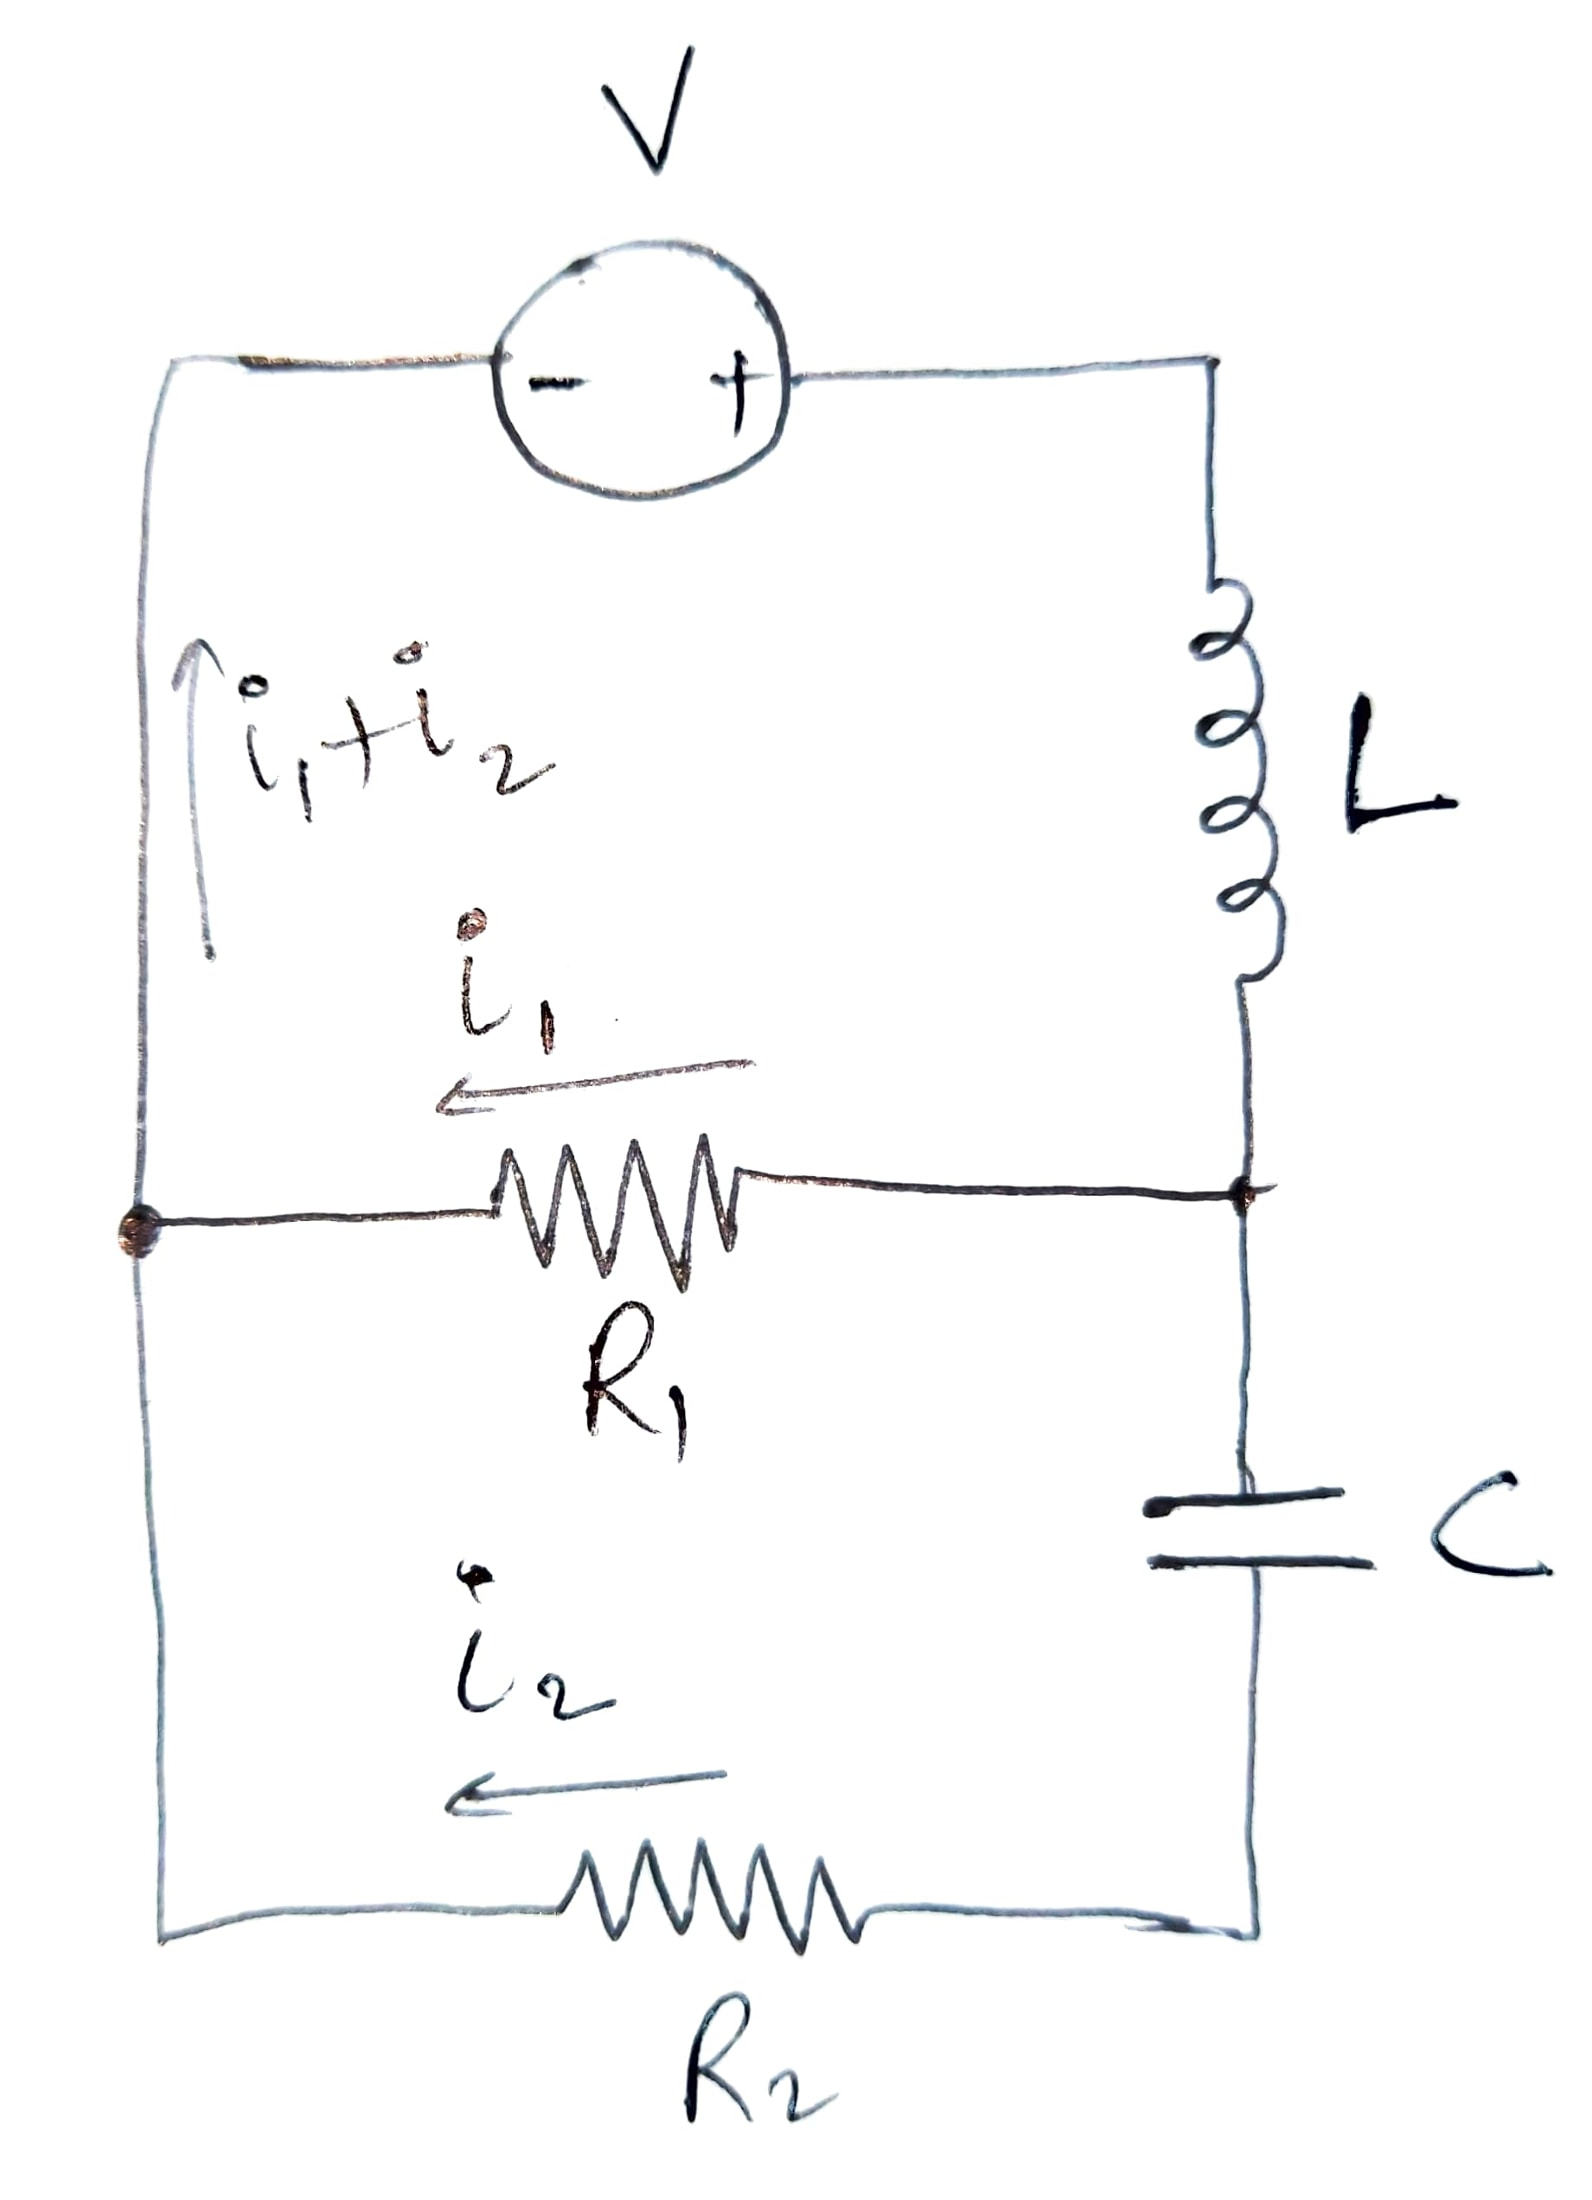
\includegraphics[height=0.5\textheight,width=\textwidth]{images/current1.jpeg}
        \vfill

		\column{0.8\textwidth}
        \begin{itemize}
            \item KVL on upper loop:
                $$
                \boxed{V - L \frac{d(i_1 + i_2)}{dt} - i_1 R_1 = 0}
                $$
            \item KVL on lower loop:
                $$
                i_1 R_1 - \frac{q_2}{C} - i_2 R_2 = 0
                $$
                $$
                \boxed{i_1 R_1 - \frac{1}{C} \int_0^ti_2 dt - i_2 R_2 = 0}
                $$
                (Assuming the initial voltage across the capacitor to be zero)
            \item Solving these two differential equations, we can find $i_1$ and $i_2$.
        \end{itemize}

	\end{columns}
\end{frame}

\begin{frame}
    \frametitle{Other physical phenomena}
    Other than the phenomena mentioned so far, all the other fields of physics use differential equations to model the physical system or phenomena. Some of the examples are:
    \begin{itemize}
        \item In Magnetism: finding magnetic field due to a varying current, effects of varying magnetic field, etc.
        \item In Fluid Mechanics: finding pressure when the density is varying, time taken for a tank to empty through a pipe, etc.
        \item In Heat Conduction and Thermodynamics: finding the time taken for a block to reach a given temperature when heated at one end, finding the heat current when the conductivity is varying with length, etc.
        \item In Planetary Motion (discussed later)
    \end{itemize}
    Modelling conservation laws and planetary motion are discussed in the upcoming slides.
\end{frame}

\section{Conservation Laws}

\begin{frame}
    \fontsize{9pt}{10pt}\selectfont
    \frametitle{Laws of Conservation}
    \framesubtitle{Definition and Types}
    A conservation law can be stated as follows:
    \begin{itemize}
        \item A particular measurable property of an isolated physical system does not change as the system evolves over time.
        \item So, the basic idea is that any particle interaction must not change the total energy, total mass, and total charge of the particles, given any condition they are in. This is also known as “the particle physics conservation laws” or “the conservation laws in nuclear physics”.
    \end{itemize}
    We study more or less the following kinds of laws of conservation:
    \begin{itemize}
        \item Mass-energy Conservation: The total mass and energy of particles before and after the exchange must be the same.
        \item Momentum Conservation: Momentum, defined as $p = mv$, where $m =$ mass of particle, $v =$ velocity of particle. The total momentum of the system’s particles before and after the impact are the same.
        \item Charge Conservation: The total charge of the particles before and after the exchange is the same.
    \end{itemize}
\end{frame}

\begin{frame}
    \frametitle{Laws of Conservation}
    \framesubtitle{Motive}
    When we formulate a mathematical model for a ‘continuum’ physical system, the following are the basic steps:

    \begin{enumerate}
        \item To identify appropriate conservation laws (eg., mass, energy, momentum, etc).
        \item Identify their corresponding densities and fluxes.
        \item Writing corresponding equations using conservation.
        \item Closing the system of equations by proposing appropriate relationships between fluxes and the densities.
    \end{enumerate}
    The first, second and fourth have physical requirements, the third one is the mathematical one and this is the one which we would be focusing on.
\end{frame}

\begin{frame}
    \fontsize{9pt}{10pt}\selectfont
    \frametitle{Laws of Conservation}
    \framesubtitle{Motive}
    Once a model is formulated, another step gets involved: -

    \begin{itemize}
        \item Analyzing and validating the model
        \item Comparing its predictions with observations
        \item Correcting them whenever needed
    \end{itemize}

    In any ‘continuum’ modeling, there are several scales:

    \begin{itemize}
        \item Visible scales: Densities and fluxes (Mathematical variables in the model vary)
        \item Invisible scales: The micro-scales that have been averaged in obtaining the model
    \end{itemize}

    For example, considering the first scale, when we talk about ‘river flow’:

    \begin{itemize}
        \item We can say that volume density (volume per unit length), $A$, as “density”, $u$ as the average flow velocity, then $Q = uA$.
        \item Here, $Q$  is the volume flux of water down the river (volume per unit time).
        \item This follows conservation of volume, since water is incompressible.
    \end{itemize}
\end{frame}

\begin{frame}
    \frametitle{Conservation forms and Differential forms}
    \begin{itemize}
        \item Now coming to the mathematical part, the conservation laws and the differential laws are inter changeable.

    $$
    u_t + (f(u))_x = 0 \quad \underleftrightarrow{(\textrm{if } u \in C^1)} \quad u_t + f'(u)u_x = 0
    $$
    where, $f =$  flux function; $f'(u) = c(u)$

        \item The equation towards left: Conservation Form

        \item The equation towards right: Differential Form


    $$
    \frac d {dt} \int\limits_{a}^{b}u(x, t)dx = f(u(a, t)) - f(u(b, t))
    $$

        \item This is the integral form.
    \end{itemize}
\end{frame}

\begin{frame}
    \frametitle{Example}
    \framesubtitle{Traffic Flow}

    \begin{itemize}
        \item Let us define: $\rho (x, t) =$  vehicle density,  $\rho = 0$, empty and $\rho = 1$, packed

    $m(t) = \int\limits_{a}^{b} \rho(x, t)dx =$  number of vehicles in $[a, b]$

        $\frac{d}{dt} m(t) = $ Influx $-$ Ouflux

        $$
        \frac d {dt} m(t) = f(\rho (a, t)) - f(\rho(b, t))
        $$


         \item Equation: $\rho_t + (f(\rho))_x = 0,$  where $f(\rho) = v.\rho,$ where $v =$  velocity.

         \item Velocity Function: $v = v(\rho) = 1 - \rho$
         \item Flux Function: $f(\rho) = \rho(1-\rho)$
         \item Velocity of Information: $c(\rho) = f'(\rho) = 1-2\rho$
    \end{itemize}
\end{frame}

\begin{frame}
    \frametitle{Conservation of Energy}
    \begin{itemize}
        \item As the First Law of Thermodynamics can be stated as:

        The total energy change in system equals the difference between the heat transferred to the system and the work done by the system on its surroundings.

        $$
        \frac {dE} {dt} = Q'-W'
        $$

        where, $Q=$ heat transfer, $W =$  work done

        \item The above equation is used when the work is assumed to be done by the system.

        \item When the work is done on the system by its surroundings, then the equation basically is:

        $$
        \frac {dE} {dt} = Q'+W'
        $$

    \end{itemize}
\end{frame}

\begin{frame}
    \frametitle{Conservation of Energy}
    \begin{itemize}
        \item The \textit{energy per unit mass} contained in a system is of three parts:

        internal, kinetic and potential. Thus, we can write the total energy equation as follows:

        $$
        e_t = e(Total) = e(Internal)+e(Kinetic)+e(Potential)
        $$

            \begin{itemize}
                \item $\space e(Internal) = e(T)$

                \item $\space e(Kinetic) = \frac 1 2 v^2$, where $v =$  velocity of the particle

                \item $\space e(Potential) = gz$, where $z =$  height, $g =$  Gravitational Acceleration
            \end{itemize}

        \item Therefore, the total energy can be written as: -

        $$
        E = \int\int\limits_{\Omega}\int \rho e_t d\Omega = \int\int\limits_{\Omega}\int\rho[e(T)+ \frac 1 2 V^2 + gz]d\Omega
        $$
    \end{itemize}
\end{frame}

\begin{frame}
    \frametitle{Conservation of Momentum}
    \begin{itemize}
        \item Newton’s First Law of Motion or the Inertial Law states that:

            \quad \quad The momentum of a system is constant if no external forces are acting on the system.

            $$
            p_1 = p_2
            $$

        \item Let $M_1$ and $M_2$ be the masses of the two particles moving in the same line of motion. Let $u_1$  and $u_2$  be the initial velocities of two particles moving in the same line of motion and let $v_1$ and $v_2$  be the final velocities of the particles after the collision of the particles, respectively.

        \item Now, as momentum, $p = Mv$, Conservation of Momentum states that

            $$
            M_1u_1 + M_2u_2 = M_1v_1 + M_2v_2
            $$
    \end{itemize}
\end{frame}

\begin{frame}
    \fontsize{9pt}{10pt}\selectfont
    \frametitle{Conservation of Momentum}
    \begin{itemize}
        \item Newton’s Second Law of Motion states that:

        \quad \quad The acceleration of an object depends upon the net force acting on the object and the mass of the object.

        \item Now, for $x =$  distance, $u =$  velocity, $a =$  acceleration, $t =$  time, $m =$  mass, $\rho =$  density, $A =$  area, $F =$ force, $p =$ pressure
        $$
        F = ma
        $$
        \item The above can be written as:
            $$
            F = ma = m \frac {du} {dt} \implies -[(pA_2) - pA_1] = m(\frac {u_2 - u_1} {dt})
            $$
            $$
            \implies -[(p + (\frac {dp} {dx})dx)A - pA = m(\frac {u + (\frac{du} {dx})dx - u} {dt})
            $$
            $[m = \rho dx A]$
            $\implies \space - (\frac {dp} {dx})dxA = m(\frac {du} {dx}) \frac {dx} {dt},$  where $\frac {dx} {dt} = u$

        Therefore, the differential form can be written as:
        $$
        -\frac {dp}{dx} = \rho u \frac {du} {dx}
        $$
    \end{itemize}
\end{frame}

\begin{frame}
    \frametitle{Conservation of Charge}
    \begin{itemize}
        \item The conservation of charge states that the electrical charges cannot be created or destroyed. Therefore, the total charges in the system always remains the same irrespective of any given condition.

        \item Integral Form:

        The integral formulation of conservation of charge is: -

        $$
        \int\limits_A j.da = -\frac {d} {dt} \int\limits_V \rho dv = -\frac {dQ}{dt}
        $$

        where,

        $j:$  current density,
        $\rho:$ volumetric charge density,
        $Q:$  total charge inside the volume,
        $A:$  surface area of the volume and
        $V:$  volume

        \item Differential Form

        The differential formulation of conservation of charge is:
        $$
        \Delta j = -\frac {d\rho}{dt}
        $$
    \end{itemize}
\end{frame}

% \begin{frame}
%     \frametitle{Conservation of charge}
%     \framesubtitle{Formula from Ampere - Maxwell's Law}
%     \begin{itemize}
%         \item The conservation of charge can be derived from the Ampere - Maxwell law and Gauss’s law for electric charges.

%         $$
%         \Delta \times h = j + \frac {d \space d}{dt}
%         $$

%         where, $j =$  free charge density
%     \end{itemize}
% \end{frame}

\section{Planetary Motion}

\begin{frame}
    \frametitle{Planetary Motion}
    \framesubtitle{Introduction}
    \begin{itemize}
        \item Ancient Greek astronomers knew the existence of five "stars", Mercury, Venus, Mars, Jupiter, and Saturn. To them, the apparent motion of these objects was following an irregular path, and was not normal compared to the observable regular pathways of the other stars. The view that the Earth was in the centre of the Universe was also deeply rooted in their religious beliefs.
        \item Copernicus, however, concluded that these planets revolve around the sun in circular orbits. Later, based on Tycho Brahe's observations, Kepler concluded that the speculated circular orbits were not in agreement with those observations, and that elliptical orbits were the answer.
    \end{itemize}
\end{frame}

\begin{frame}
    \frametitle{Kepler's Laws}
    Based on the motion of the planets about the sun, Kepler devised a set of three classical laws, called Kepler’s laws of planetary motion, that describe the orbits of all bodies satisfying these two conditions:
    \begin{itemize}
        \item The orbit of each planet around the sun is an ellipse with the sun at one focus.
        \item Each planet moves so that an imaginary line drawn from the sun to the planet sweeps out equal areas in equal times.
        \item The ratio of the squares of the periods of any two planets about the sun is equal to the ratio of the cubes of their average distances from the sun.
    \end{itemize}
\end{frame}

\begin{frame}
    \fontsize{9pt}{10pt}\selectfont
    \frametitle{Derivation of the Orbit}
    Newton’s Universal Law of Gravitation states that the gravitational force between the Sun M and a planet m is proportional to the product of the two masses and inversely proportional to the distance between them. Gravity is an attractive force. Therefore, M pulls m towards itself.
	\begin{columns}
		\column{0.35\textwidth}
        \centering
        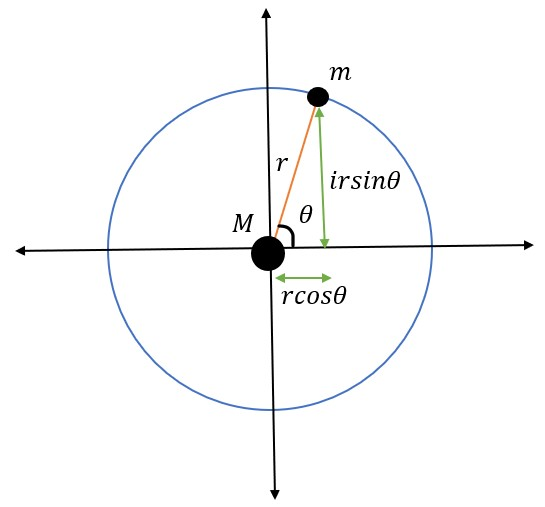
\includegraphics[height=0.4\textheight,width=\textwidth]{images/1.jpg}
        \vfill

		\column{0.8\textwidth}
        \begin{center}
           $F=-G\frac{mM}{r^2}$
        \end{center}
        From Newton's Second Law of Motion,
        \begin{equation}
               a=-G\frac{M}{r^2}e^{i\theta}
        \end{equation}
        We also have,
        $$
        z(t)=re^{i\theta} \implies
        v(t)=\frac{dz}{dt}=ire^{i\theta}\frac{d\theta}{dt}+e^{i\theta}\frac{dr}{dt}
        $$
        \begin{equation}
        a(t)=e^{i\theta}(-r(\frac{d\theta}{dt})^2+\frac{d^2r}{dt^2}+i( \frac{d}{dt}(r^2\frac{d\theta}{dt})))
        \end{equation}
	\end{columns}
\end{frame}

\begin{frame}
    \frametitle{Derivation of the Orbit (cont.)}
    Equating real and imaginary parts of (1) and (2):
    \begin{equation}
        G\frac{M}{r^2}=-r(\frac{d\theta}{dt})^2+\frac{d^2r}{dt^2}
    \end{equation}
    \begin{equation} \frac{d}{dt}(r^2\frac{d\theta}{dt})=0
    \end{equation}
    From equations (3) and (4), we get the $2^{nd}$ order ODE of the orbit ($r=\frac{1}{s}$ and c is a constant)
    \begin{center}
        $\frac{d^2s}{d\theta^2}=-s+\frac{GmM}{c^2}$
    \end{center}
    The solution for this equation will be of the form
    \begin{equation}
        s=Asin\theta+Bcos\theta+\frac{GmM}{c^2}
    \end{equation}
\end{frame}

\begin{frame}
    \frametitle{Derivation of the Orbit (cont.)}
    To simplify the equation, we assume that M and m are the closest to each other when m is on the positive real axis. That means, s has a local maximum at $\theta=0$
    $\implies \frac{ds}{d\theta}=0$ and $\frac{d^2s}{d\theta^2} \leq 0$\\
    This gives us our final equation:
    \begin{center}
        $s=Bcos\theta+\frac{GmM}{c^2}$ where $B\leq0$
    \end{center}
    \begin{center}
        $\frac{1}{r}=Bcos\theta+\frac{GmM}{c^2}\implies r=\frac{c^2/GmM}{1+(c^2B/GmM)cos\theta}$
    \end{center}
    Let $a=c^2/GmM$ and $e=aB$. Then,
    \begin{center}
        $r=\frac{a}{1+ecos\theta}$ \\
    \end{center}
    where a is the semi-major axis and e is the eccentricity of the ellipse.
\end{frame}

\section{Conclusion}

\begin{frame}
    \frametitle{Conclusion}
    \begin{itemize}
        \item We see that almost every system or phenomena shown in this presentation has differential equations to represent the behaviour and other parameters. By studying differential equations and the ways to analyze or solve them, we are learning how to analyze real world phenomena, and ways to solve real world problems.
        \item From the above slides, we can conclude that differential equations have significant amount of role in deriving and stating various physical phenonmenon, laws of conservation, planetary motion and various other phenonmenon.
    \end{itemize}
\end{frame}

% \begin{frame}
%     \frametitle{dummy}
%     \begin{itemize}
%         \item Ref: \cite{modelling_phy_sys_with_linear_de}
%         \item Ref: \cite{papadatos2016equations}
%         \item Ref: \cite{hsu2018applied}
%         % \item Ref: \cite{howard2009modeling}
%         \item Ref: \cite{rosales2002conservation}
%         \item Ref: \cite{chaachoua2006modelling}
%         \item Ref: \cite{kep_new_planet}
%         % \item Ref: \cite{enwiki:1059423382}
%         % \item Ref: \cite{enwiki:1078412066}
%         % \item Ref: \cite{enwiki:1080187787}
%     \end{itemize}
% \end{frame}

\begin{frame}
    \fontsize{8pt}{9pt}\selectfont
    \frametitle{References}
    \printbibliography
\end{frame}

\begin{frame}
    \begin{center}
        \huge Thank You!
    \end{center}
\end{frame}

\end{document}
